\section{Antenna Tipping}

\subsection{Marco teórico}

La turbulencias atmosféricas y el vapor de agua presente en la atmósfera distorsionan la señal de un objeto celeste dando lugar a un error sistemático que no depende del radiotelescopio.

La atmósfera en sus distintas capas varía la temperatura y la densidad pero en este experimento se hace una aproximación a primer orden para establecer que contribuye una temperatura de ruido $T_\textnormal{atm}$ fija. Además, se hace también una aproximación al igualar la temperatura ambiente del domo $T_\textnormal{amb}$ con $T_\textnormal{atm}$.

La opacidad cenital $\tau_\textnormal{w}$ debido al contenido de agua en la atmósfera y la opacidad cenital total $\tau_0$ de la atmósfera, que incluye al oxígeno, se aproximan también a primer orden para decir que son iguales.

El método Antenna Tipping permite calibrar el receptor del telescopio al determinar el estado y opacidad cenital de la atmósfera.

Se mide la potencia del cielo $W_\textnormal{sky}$ detectada por el telescopio a un determinado intervalo de frecuencias y elevación $\varphi$, que está dada por,
\begin{equation}
W_\textnormal{sky}=c\left(T_\textnormal{rec}+T_\textnormal{atm}\left(1-\exp\left(-\tau_\textnormal{0}/\sin\varphi\right)\right)\right)
,\end{equation}
donde $T_\textnormal{rec}$ es la temperatura de ruido del receptor y $c$ es una constante que, por ejemplo, puede depender de la ganancia del receptor.

Análogamente, la potencia para una carga enfrente de la bocina a temperatura ambiente $T_\textnormal{amb}$ (la misma carga Hot del Hot--Cold Test), la potencia es,
\begin{equation}
W_\textnormal{amb}=c\left(T_\textnormal{rec}+T_\textnormal{amb}\right)
.\end{equation}

Aplicando las aproximaciones, se define,
\begin{equation}
\Delta W\equiv W_\textnormal{amb}-W_\textnormal{sky}=cT_\textnormal{amb}\exp(-\tau_\textnormal{w}/\sin\varphi)\label{eq:deltaw}
,\end{equation}
y $z=\pi/2-\varphi$, permitiendo obtener la relación,
\begin{equation}
\ln\left(\Delta W\right)=-\sec\left(z\right)\tau_\textnormal{w}+\ln\left(cT_\textnormal{amb}\right)\label{eq:taufit}
,\end{equation}
que es una relación lineal de $\ln(\Delta W)$ con respecto a ${-\sec\left(z\right)}$, donde $\tau_\textnormal{w}$ es la pendiente de la recta.

\subsection{Datos y metodología}

Se utiliza una carga caliente a temperatura ambiente en la cúpula del radiotelescopio MINI, midiendo la potencia que muestra Domo en la tabla \ref{tab:taufit}.

Se mide con un \textit{powermeter} la potencia espectral de diez puntos a distintas elevaciones y azimut fijo, entregando los resultados de la tabla \ref{tab:taufit}.
\begin{table}[htbp]
	\centering
	\begin{tabular}{
			@{}
			l
			S[table-format=2.2]
			S[table-format=2.2]
			@{}
		}
		\toprule
		{Punto} &
		{Elevación} &
		{Potencia} \\
		{} &
		{\textdegree} &
		{\si{\dBm}} \\
		\midrule
		1 & 23.50 & -45.56 \\
		2 & 16.60 & -45.22 \\
		3 & 12.84 & -45.01 \\
		4 & 10.48 & -44.88 \\
		5 & 8.85 & -44.80 \\
		6 & 7.66 & -44.73 \\
		7 & 6.76 & -44.71 \\
		8 & 6.04 & -44.67 \\
		9 & 5.47 & -44.65 \\
		10 & 4.99 & -44.63 \\
		Domo & & -44.54 \\
		\bottomrule
	\end{tabular}
	\caption{Elevación y potencia para los distintos puntos a azimut fijo. Se incluye domo con carga caliente}\label{tab:taufit}
\end{table}

\subsection{Cálculo de $\tau_\textnormal{w}$}

El siguiente procedimiento corresponde al código \ref{cod:antennadipping}. Se lee el archivo \texttt{antdip\_AE2021A} provisto por el equipo docente con los datos necesarios para realizar el ajuste lineal según la ecuación \ref{eq:taufit}. El gráfico de este se muestra en la figura \ref{fig:taufit}. La pendiente de la recta establece un valor de \num{0.2573501} para la opacidad cenital debido al contenido de agua en la atmósfera.

\begin{figure}[htbp]
	\centering
	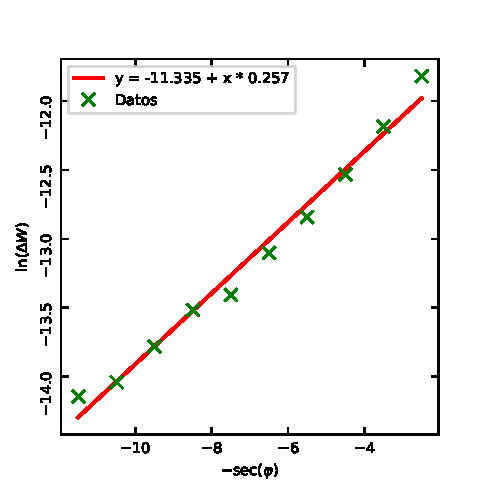
\includegraphics{taufit.pdf}
	\caption{Equis roja es medición del telescopio. Línea azul es ajuste lineal. La pendiente es $\tau_\textnormal{w}$}
	\label{fig:taufit}
\end{figure}

\subsection{Comparación con calibración del MINI}

El software del MINI tiene el comando \texttt{\%antdip} para ingresar todo el sistema a una subrutina de Antenna Dipping.

Primeramente se debe ingresar la cantidad de masas de aire por punto y se usa \num{1}, que es el valor típico.

Luego el sistema recolecta automáticamente información para diez puntos separados por una masa de aire a través de la elevación a azimut fijo, midiendo la mayor elevación primero y luego disminuye progresivamente. El telescopio constantemente evalúa su posición y solo toma datos cuando está apuntando con cierta tolerancia a la coordenada determinada por el sistema de control.

La información recolectada corresponde a la diferencia de potencia de la ecuación \ref{eq:deltaw}, donde la potencia para el cielo es la que apunta según la elevación correspondiente y la potencia para la carga caliente es según el \textit{chopper}, una carga absorbente electromagnética, que está dentro de la bocina de la antena y automática y periódicamente obstruye la visión del telescopio gracias a un motor.

Tras medir los diez puntos, automáticamente el telescopio apunta al domo y toma una medición de referencia con la carga caliente. A continuación, se debe ingresar la temperatura actual y la humedad relativa, además de un parámetro cualitativo de \num{0} a \num{3} que indica el grado de cobertura del cielo debido a las nubes y sirve para el registro histórico.

Finalmente, el software realiza el ajuste lineal y entrega el valor $\tau_\textnormal{w}'=\num{0.2573501}$, además de otros parámetros como la estimación de la eficiencia del telescopio y la temperatura de brillo del agua en el cielo.

Se aprecia que $\tau_\textnormal{w}=\tau_\textnormal{w}'$.